\documentclass[twocolumn,english]{article}
\usepackage[latin9]{inputenc}
\usepackage[landscape]{geometry}
\geometry{verbose,tmargin=0.5in,bmargin=0.75in,lmargin=0.5in,rmargin=0.5in}
\setlength{\parskip}{0bp}
\setlength{\parindent}{0pt}
\usepackage{color}
\usepackage{float}
\usepackage{amstext}
\usepackage{graphicx}
\PassOptionsToPackage{normalem}{ulem}
\usepackage{ulem}

\makeatletter



\usepackage{array}
\usepackage{multirow}
\usepackage{amsbsy}




\providecommand{\tabularnewline}{\\}

\setlength{\columnsep}{0.25in}
\usepackage{xcolor}
\usepackage{textcomp}
\usepackage{listings}
\lstset{
  tabsize=2,
  basicstyle=\small\ttfamily,
}



\usepackage{babel}
\usepackage{listings}
\renewcommand{\lstlistingname}{Listing}

\makeatother

\usepackage{babel}
\usepackage{listings}
\renewcommand{\lstlistingname}{Listing}

\begin{document}

\title{Reference Sheet for C220 Software Engineering Design}

\date{Autumn 2017}
\maketitle

\section{Test-Driven Development}

\paragraph{TDD Cycle}
\begin{enumerate}
\item Write a failing test (API design).
\item Code to pass test (internals design).
\item Refactor (structural design).
\end{enumerate}

\paragraph{Refactoring}

Process of improving the design of a piece of code, without changing
its functionality.
\begin{itemize}
\item Should be applied \emph{little and often} to continuously improve
design.
\item Only refactor in a \emph{green state}. Tests ensure that behaviour
is preserved.
\item Should be \emph{automated} to be done quickly and reliably.
\item Small transformations are \emph{combined} to achieve larger refactorings.
\end{itemize}

\paragraph{Example Transformations}
\begin{enumerate}
\item \emph{Compose (extract) method}: Break down method into chunks to
make it shorter. Allows us to give a name for a concept and increase
level of abstraction. Try to keep a constant level of abstraction.
\item \emph{Inline variable}: Instead of using a temporary variable, inline
its usages. Reduces number of elements in method.
\item \emph{Extract to common class}: First work to make duplication exactly
the same. Then refactor it, e.g. to another object. Reduces duplication.
\end{enumerate}

\paragraph{Technical Debt}

Features are been added quickly, in an inelegant way. When not fixed
quickly, \emph{technical debt} builds up.

\subsubsection*{JUnit and JMock}

\begin{lstlisting}[language=Java,basicstyle={\footnotesize\ttfamily},commentstyle={\color{gray}\itshape}]
public class TestObjectTest {
  // Set up mockery, constants, mock objects and tested object
  @Rule public JUnityRuleMockery context = new JUnitRuleMockery();

  final Order EXAMPLE_PARAM = new ...;

  CalledObject calledObject = context.mock(CalledObject.class);
  ...

  TestObject testObject = new TestObject(calledObject, ...)

  @Test
  public void doesSomethingSpecific() {
    // Set up local variables for exceptions / return values
    SomeException exception = new SomeException();

    // Set up expectations
    context.checking(new Expectations() {{
      // Ignore: ignoring / allowing
      ignoring(unimportantMockObject);
      allowing(someMockObject).someMethod(with(any(ParamType.class)));
                               will(throwException(exception));

      // Expect: exactly(n) / atLeast(n) / atMost(n)
      exactly(1).of(anotherMockObject).someOtherMethod(exception);
      exactly(1).of(anotherMockObject).anotherMethod(EXAMPLE_PARAM);
                                       will(returnValue(x));

      // Don't expect: never
      never(aDifferentMockObject).aDifferentMethod();
    }});
    
    // Set up triggers
    testObject.testedMethod(EXAMPLE_PARAM, ...);
    testObject.anotherTestedMethod();

    // Make assertions
    assertThat(testObject.getSomeValue(), is(x));
  }
}
\end{lstlisting}

\section{UML Diagrams}

\subsubsection*{UML Class Diagrams}

\begin{figure}[H]
\centering{}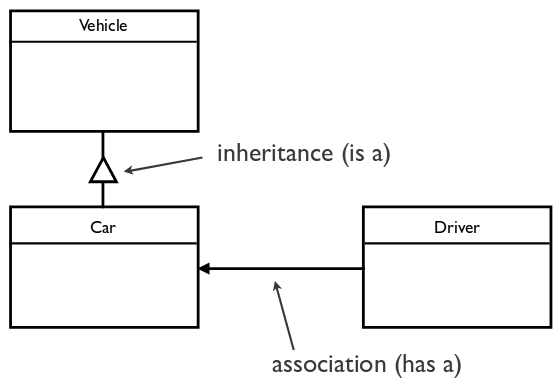
\includegraphics[width=0.35\columnwidth]{img/uml-class}
\end{figure}

\subsubsection*{UML Object Diagrams}

\begin{figure}[H]
\centering{}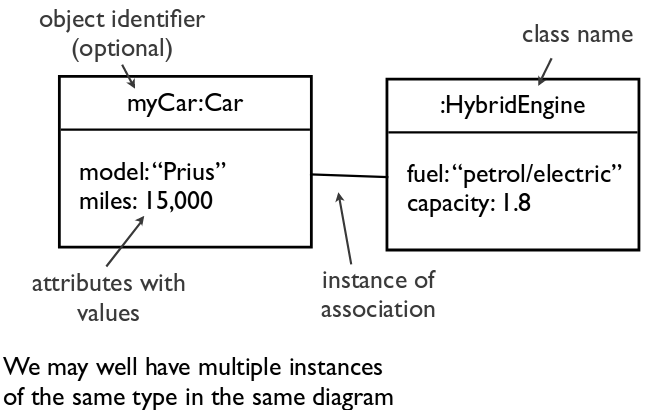
\includegraphics[width=0.4\columnwidth]{img/uml-object}
\end{figure}

\subsubsection*{UML Sequence Diagrams}

\begin{figure}[H]
\centering{}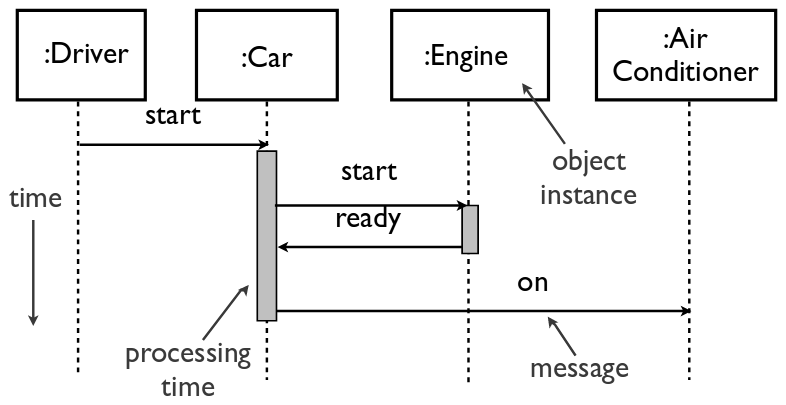
\includegraphics[width=0.5\columnwidth]{img/uml-sequence}
\end{figure}

\section{Object Oriented Design}

\paragraph{Four Elements of Simple Design}

In order of importance:
\begin{enumerate}
\item Behaves correctly.
\item Minimises duplication.
\item Maximises clarity.
\item Has fewer elements.
\end{enumerate}

\paragraph{Bad Design}
\begin{itemize}
\item \emph{Rigidity}: software is hard to change.
\item \emph{Fragility}: when we change one part, other parts break unexpectedly.
\item \emph{Immobility}: it is hard to reuse elements of the code in other
applications.
\end{itemize}

\paragraph{Commands vs. Queries}
\begin{itemize}
\item \emph{Commands}:\emph{ Ask another object to do something for us}.
Don't care how it's done, don't expect return value. Changes state
of invoked object.
\item \emph{Queries}:\emph{ Ask another object to tell us a value} (so we
can do something with it). Should return value, but not have side
effects on state of invoked object.
\end{itemize}

\paragraph{Tell Don't Ask}

Objects send messages, requesting actions, but do not expect return
values. Only queries return values.

\paragraph{Law of Demeter}

\emph{Only talk to your immediate friends}. Implementations that depend
on pieces of the system further away result in tight coupling.

Avoid \emph{train wrecks}: \texttt{getX().getY().getZ().doSomething()}.

\paragraph{Visibility}
\begin{itemize}
\item \emph{Encapsulation}: ensure object's behaviour is only affected through
its API. Implementation and state of objects should be encapsulated.
Reduces fragility.
\item \emph{Information hiding}: conceal how an object implements functionality.
Increases abstraction, chunking up program into concepts.
\end{itemize}
\emph{Key idea}: Make things \texttt{private} unless they should exposed
as an API for other objects (and generally avoid \texttt{protected}).

\paragraph{Coupling and Cohesion}
\begin{itemize}
\item \emph{Coupling}: How dependent two classes are towards each other.
Reducing coupling reduces fragility and allows reuse.
\item \emph{Cohesion}: An object should have one basic responsibility. Increasing
cohesion makes objects easier to reason about and reuse.
\end{itemize}
We can reduce coupling by using interfaces as roles.

\section{Design Patterns}

\subsection{Behavioural Patterns}

\subsubsection{Null Object Pattern}

\paragraph{Problem}

Checking for null is ugly.

\paragraph{Solution}

Use an interface and add a Null Object class that does nothing.

\subsubsection*{Example}

\begin{figure}[H]
\centering{}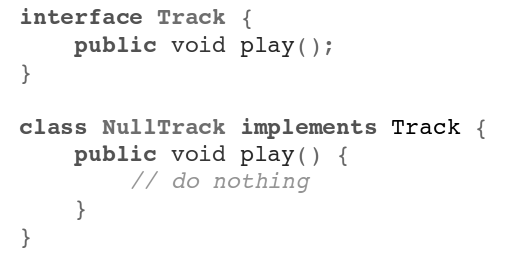
\includegraphics[width=0.4\columnwidth]{img/null-object}
\end{figure}

\subsubsection{Template Method Pattern}

\paragraph{Problem}

Requirements change over time, sometimes we need to adapt a small
part of an algorithm.

\paragraph{Solution}

Extend via inheritance.

\subsubsection*{Example}

\begin{figure}[H]
\centering{}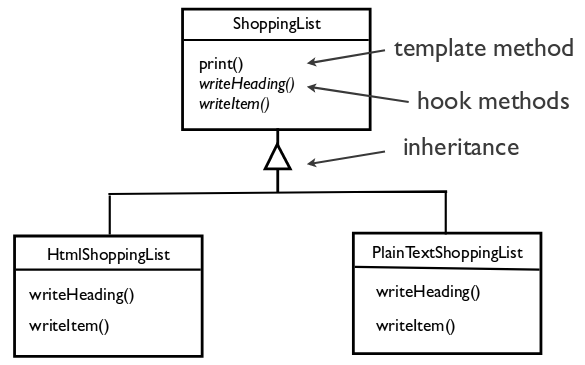
\includegraphics[width=0.5\columnwidth]{img/template-method}
\end{figure}

\paragraph{Benefits}
\begin{itemize}
\item Follows \emph{Hollywood Principle }(don't call us, we'll call you):
Concrete classes only define methods that are called when the superclass
needs them (they don't call up).
\item Follows \emph{Open-Closed Principle}: You should be able to extend
a class's behaviour without modifying it.
\begin{itemize}
\item Change behaviour by adding new code, rather than changing existing
code.
\item \emph{Separate things that change from things that stay the same}.
\end{itemize}
\end{itemize}

\paragraph{Drawbacks}

Immobility caused by coupling.

\subsubsection{Strategy Pattern}

\paragraph{Problem}

Requirements change over time, sometimes we need to adapt a small
part of an algorithm.

\paragraph{Solution}

Extend via delegation.

\subsubsection*{Example}

\begin{figure}[H]
\centering{}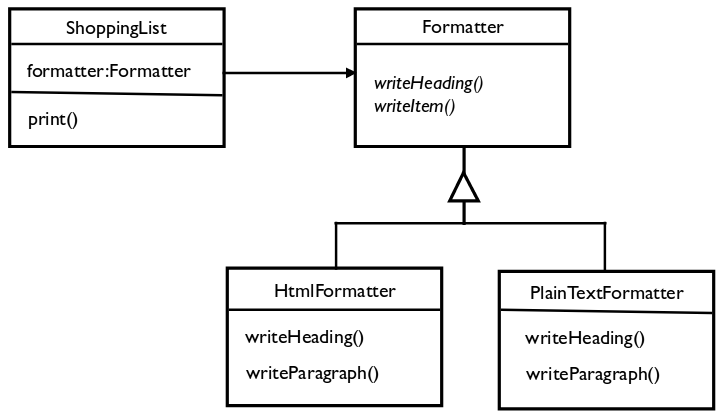
\includegraphics[width=0.6\columnwidth]{img/strategy}
\end{figure}

\paragraph{Benefits}

Does the same as the template method but with looser coupling.

\subsubsection{Observer Pattern}

\paragraph{Problem}

E.g. do $X$ when someone presses button $Y$.

\paragraph{Solution}

Subscribe to changes of state.

\subsubsection*{Example}

\begin{figure}[H]
\centering{}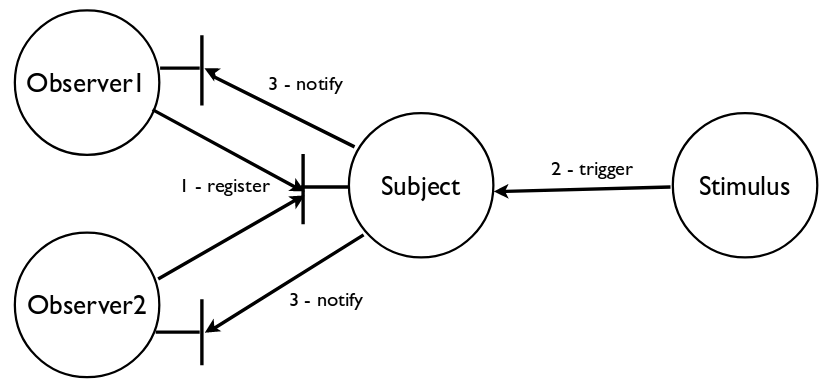
\includegraphics[width=0.6\columnwidth]{img/observer}
\end{figure}

\subsubsection{Command Pattern}

\paragraph{Problem}

Want to queue / log executed commands.

\paragraph{Solution}

Wrap up a piece of behaviour to do now or later, in an object.

\subsubsection*{Example}

\begin{figure}[H]
\centering{}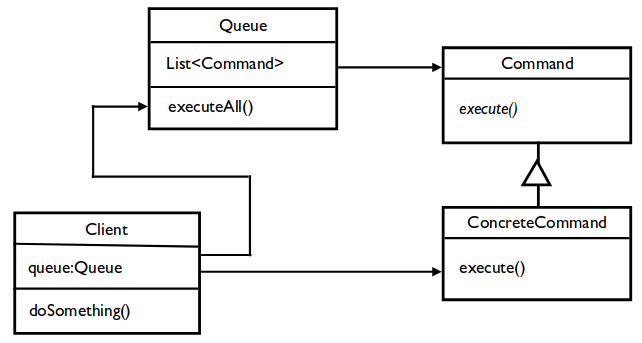
\includegraphics[width=0.5\columnwidth]{img/command}
\end{figure}

\subsection{Creational Patterns}

\subsubsection{Factory Pattern}

\paragraph{Problems}
\begin{itemize}
\item Constructors are not clear.
\item Required type may not be known until runtime.
\end{itemize}

\paragraph{Solution}

Name constructors.

\subsubsection*{Examples}

\begin{figure}[H]
\centering{}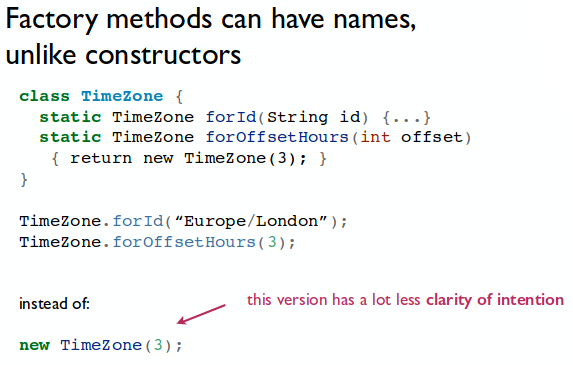
\includegraphics[width=0.45\columnwidth]{img/factory}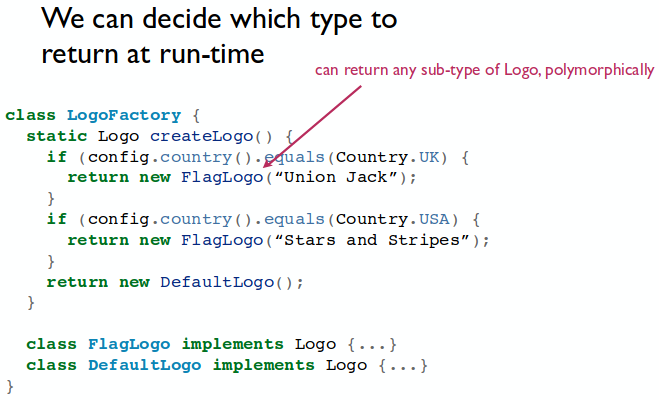
\includegraphics[width=0.5\columnwidth]{img/factory2}
\end{figure}

\subsubsection{Builder Pattern}

\paragraph{Problem}

May be many constructor parameters.

\paragraph{Solution}

Collect object's configuration parameters.

\subsubsection*{Example}

\begin{figure}[H]
\centering{}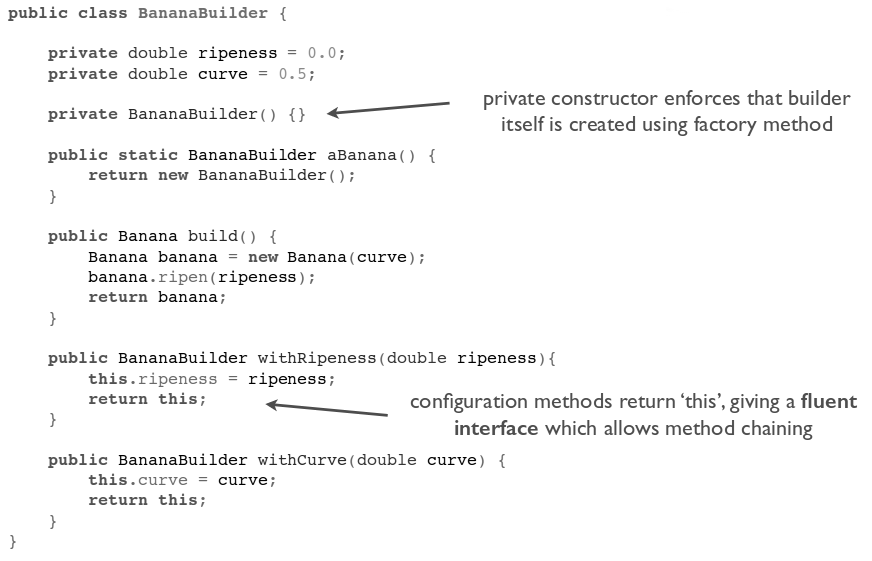
\includegraphics[width=0.55\columnwidth]{img/builder}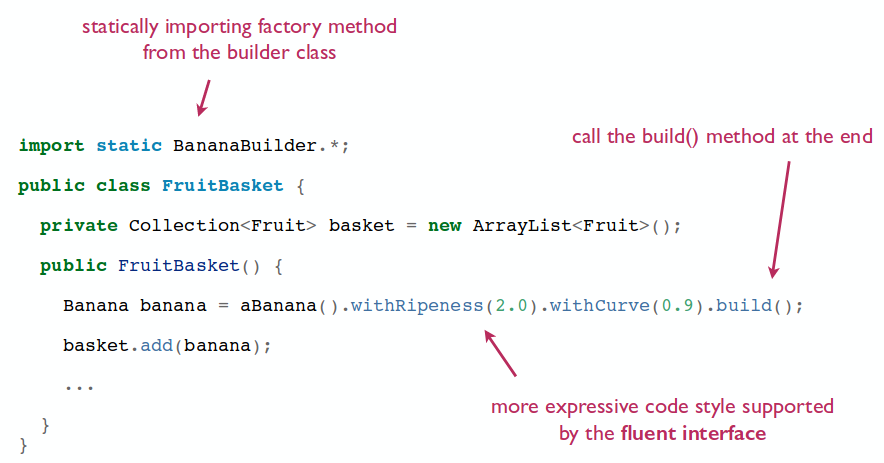
\includegraphics[width=0.45\columnwidth]{img/builder2}
\end{figure}

\subsubsection{Singleton Pattern}

\paragraph{Problem}

\emph{Require} that you only have one of a type of object.

\paragraph{Solution}

Keep a single instance and make the constructor private.

\subsubsection*{Example}

\begin{figure}[H]
\centering{}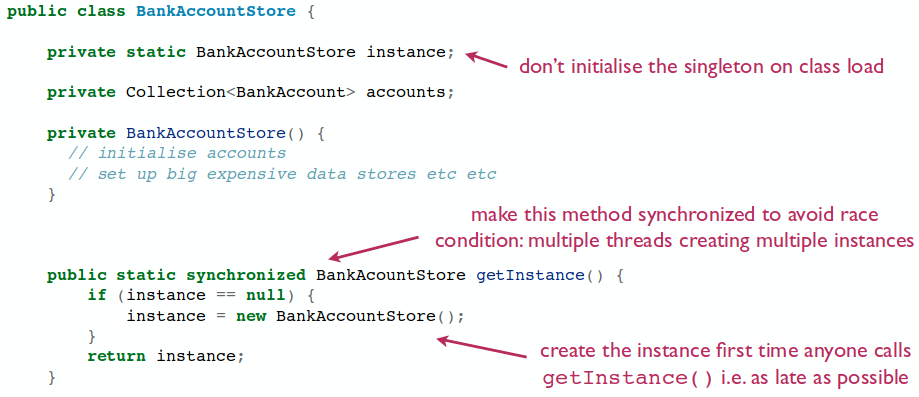
\includegraphics[width=0.6\columnwidth]{img/singleton}
\end{figure}

\paragraph{Drawbacks}

Accessing object requires tight coupling.

\subsection{Structural Patterns}

\subsubsection{Adapter Pattern}

\paragraph{Problem}

Have an $X$ but need a $Y$. E.g. translate a message from a common
format used in a message bus.

\subsubsection*{Example}

\begin{figure}[H]
\centering{}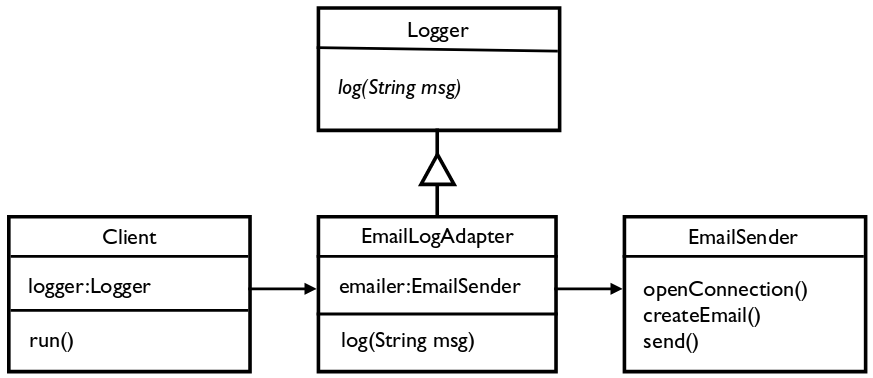
\includegraphics[width=0.6\columnwidth]{img/adapter}
\end{figure}

\subsubsection{Decorator Pattern}

\paragraph{Problem}

Have an $X$ but want a better $X$.

\subsubsection*{Example}

\begin{figure}[H]
\centering{}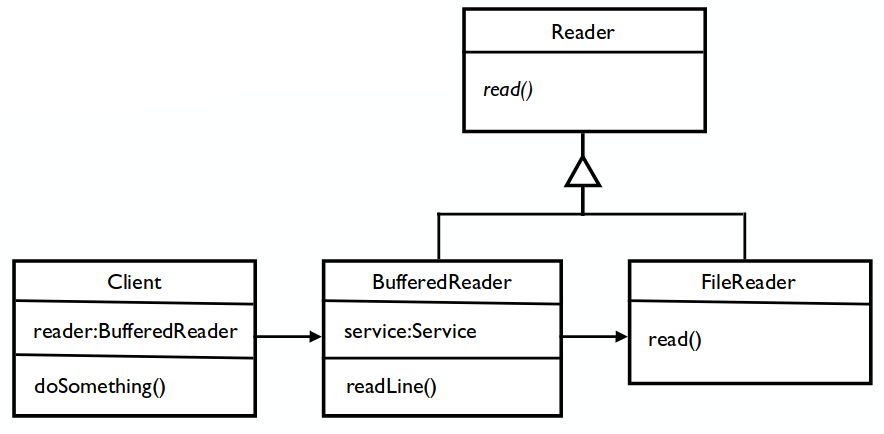
\includegraphics[width=0.6\columnwidth]{img/decorator}
\end{figure}

\subsubsection{Facade Pattern}

\paragraph{Problem}

Have an $X$ but want a simpler $X$.

\subsubsection*{Example}

\begin{figure}[H]
\centering{}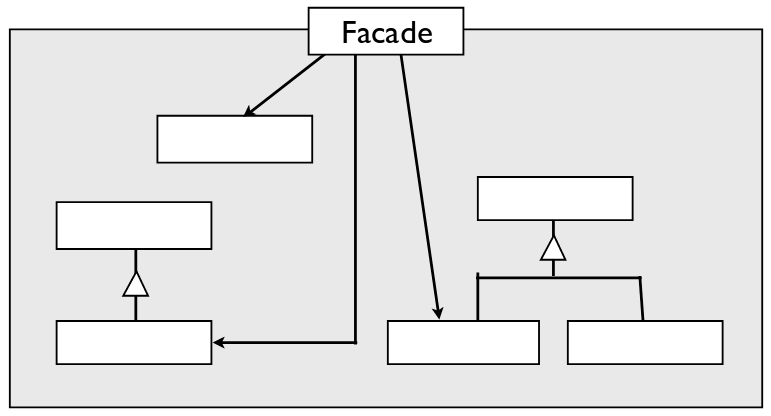
\includegraphics[width=0.4\columnwidth]{img/facade}
\end{figure}

\subsubsection{Proxy Pattern}

\paragraph{Problem}

I have an $X$ but it's too slow.

\paragraph{Solution}

Control access to a surrogate object.

\subsubsection*{Example}

\begin{figure}[H]
\centering{}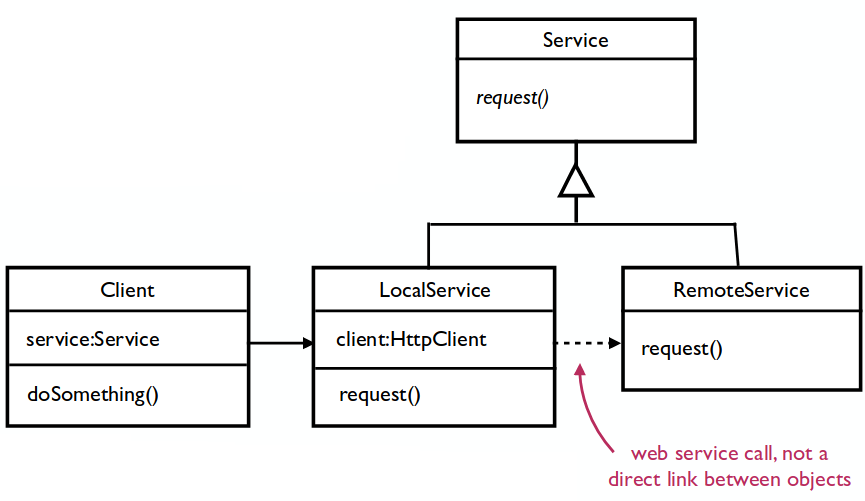
\includegraphics[width=0.6\columnwidth]{img/proxy}
\end{figure}

\paragraph{Extensions}

\emph{Caching} can reduce latency of subsequent calls.

\subsection{Architectural Styles}

\subsubsection{Model-View-Controller}

\paragraph{Problem}

Same data but different views.

\paragraph{Solution}

Separation of concerns in interactive apps.

\subsubsection*{Example}

\begin{figure}[H]
\centering{}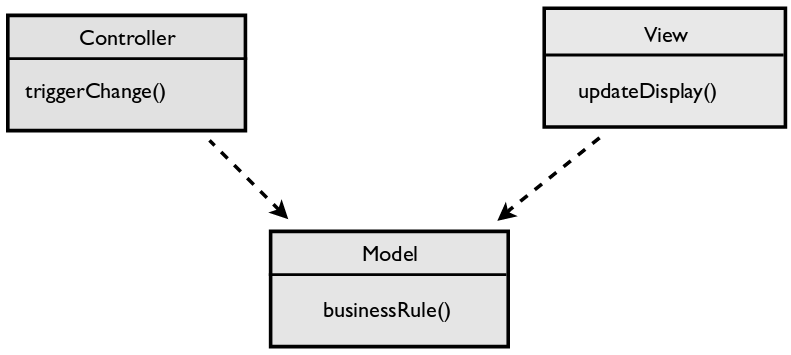
\includegraphics[width=0.45\columnwidth]{img/mvc}
\end{figure}

\subsubsection{Presentation-Abstraction-Control}

\paragraph{Problem}

GUIs with hierarchical structure.

\paragraph{Solution}

Define a tree of MVC agents that communicate up and down.

\subsubsection*{Example}

\begin{figure}[H]
\centering{}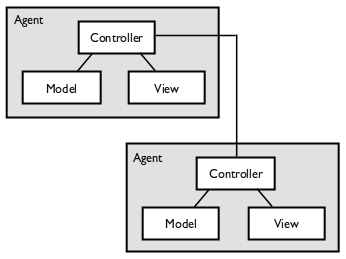
\includegraphics[width=0.4\columnwidth]{img/pac}
\end{figure}

\paragraph{Alternative}

Use an event bus to allow communication between all agents.

\subsubsection{Publish-Subscribe Pattern}

\paragraph{Problem}

Producers and consumers / balancing load.

\paragraph{Solution}

Keep a queue of commands.

\subsubsection*{Example}

\begin{figure}[H]
\centering{}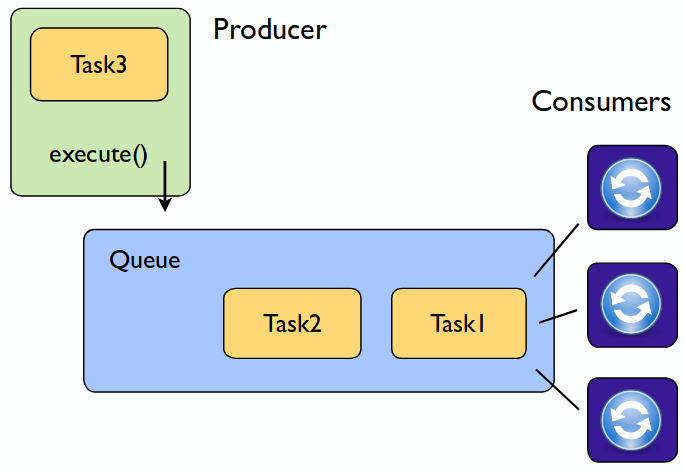
\includegraphics[width=0.4\columnwidth]{img/pubsub}
\end{figure}

\subsubsection{Map-Reduce Pattern}

\paragraph{Problem}

Large scale data processing.

\paragraph{Solution}

Divide computation into map and reduce phases to allow easy parallelisation.

\subsubsection*{Example}

\begin{figure}[H]
\centering{}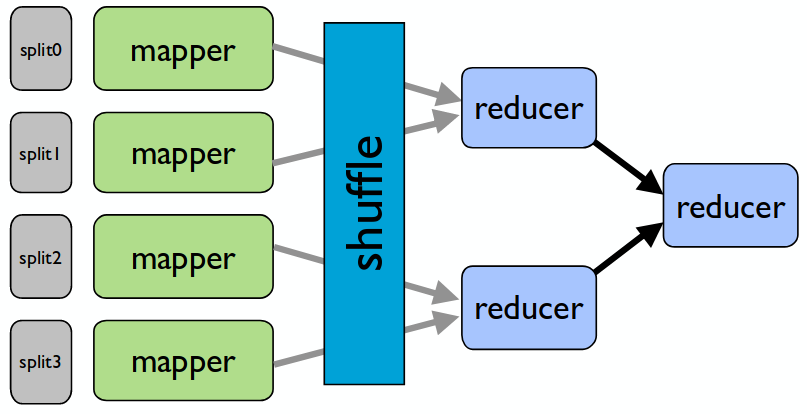
\includegraphics[width=0.4\columnwidth]{img/mapreduce}
\end{figure}

\subsubsection{Ports and Adapters / Hexagonal Architecture}

\begin{figure}[H]
\centering{}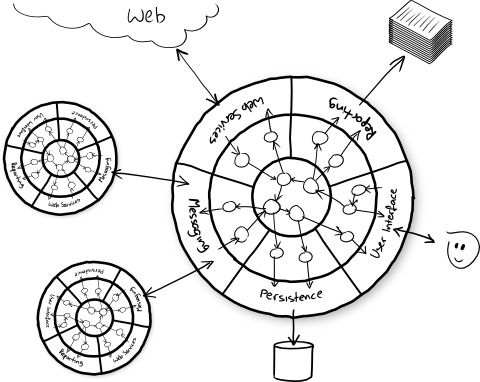
\includegraphics[width=0.5\columnwidth]{img/hexagonal}
\end{figure}
\begin{itemize}
\item Separate core application logic from services which the application
depends on.
\item Access other services only through adapters.
\item \emph{Unit test} individual objects, mocking external services at
the adapter level.
\item \emph{Integration test} the adapters.
\item \emph{System tests} run a small set of end-to-end test scenarios.
\end{itemize}

\section{Metrics}

\paragraph{Coupling}
\begin{itemize}
\item \emph{Afferent coupling}: How many other classes use (\uline{a}rrive
at) this class (measures \emph{responsibility}).
\item \emph{Efferent coupling}: How many classes are used by (\uline{e}xit)
this class (measures \emph{independence}).
\item \emph{Instability}: $\text{Ce}/\left(\text{Ce}+\text{Ca}\right)$.
Core parts should be stable. Parts at the edges, e.g. UI, don't need
to be.
\end{itemize}

\paragraph{Cyclomatic Complexity}
\begin{itemize}
\item Counts nodes and edges in the control flow of a program (number of
possible different executions).
\item Gives lower bound on number of tests required.
\end{itemize}

\paragraph{WILT}

Whitespace Integrated over Lines of Text is strongly correlated with
cyclomatic complexity.

\paragraph{ABC Metrics}

Counts occurrences of:
\begin{itemize}
\item \uline{A}ssignments
\item \uline{B}ranches
\item \uline{C}onditions
\end{itemize}
\emph{Flog} is an ABC metric tailored to Ruby. \emph{Flay} identifies
duplication.

\paragraph{Lifeline}

Graph complexity over time.

\paragraph{Turbulence}

Number of commits made to each file, compared against complexity of
code.

\section{Legacy Systems}

\emph{Legacy system}: software you have inherited and that is of value
to you.

\paragraph{Key Ideas}
\begin{itemize}
\item \emph{Understand system structure}: dependency graphs / dependency
structure matrices.
\item \emph{Preserve existing behaviour}: keep stuff that works and don't
change too much.
\item \emph{Test harness}: introduce automated tests around any changes
you make.
\begin{itemize}
\item \emph{Seams}: place where you can alter behaviour without editing
it in that place.
\item Every seam has an \emph{enabling point}: place whee you can make the
decision to use one behaviour or another.
\item \emph{Sensing}: verify correct calls are made when we can't access
values our code computes.
\end{itemize}
\end{itemize}

\section{Concurrency}

\paragraph{Key Ideas}

Try to separate code that manages threads and concurrent execution.
\begin{itemize}
\item Implementing \texttt{Runnable} instead of extending \texttt{Thread}
reduces coupling.
\item \texttt{Runnable}s can be run synchronously or asynchronously.
\item \texttt{Callable}s can also return values and throw exceptions.
\item \texttt{Execcutor}s can maintain a queue of commands. Queues can act
as load balancers.
\item \texttt{Future}s allow us to wait for a result.
\item \texttt{ExeccutorService}s allow us wait for all tasks to complete
(or use a latch).
\end{itemize}

\section{Interactive Applications}

\paragraph{Graphical User Interfaces}
\begin{itemize}
\item \emph{Use} a \texttt{JFrame} (rather than \emph{extending} it).
\item Define a \texttt{JPanel}, to which we \texttt{add} \texttt{JButton}s,
\texttt{JTextField}s, .... 
\item Add the panel to the frame using \texttt{frame.getContentPane().add(panel)}.
\item Make the window appear using \texttt{frame.setVisible(true)}.
\end{itemize}

\paragraph{Observers}
\begin{itemize}
\item Use anonymous inner classes to implement \texttt{ActionListener}s.
E.g.
\begin{lstlisting}
button.addActionListener(new ActionListener() {
	public void actionPerformed(ActionEvent actionEvent) {
		// ... do something ...
	}
});
\end{lstlisting}
\end{itemize}

\section{Web Applications}

\paragraph{Key Ideas}
\begin{itemize}
\item \emph{Serve data rather than pages}: providing an API. We can then:
\begin{itemize}
\item Process and render (e.g. using AJAX) the data (to many clients).
\item Use it in another server side application.
\end{itemize}
\item \emph{Model} often involves business logic, data from DBs, etc.
\item \emph{Controller} has to handle \emph{Routing} / \emph{parameters}
/ GET and POST \emph{requests}.
\item Provide \emph{views} (templates) for different clients.
\item \emph{Cloud} hosting often preferred to minimise responsibility/downtime
and adapt quickly to demand.
\end{itemize}

\section{Distribution and Remoting}

\paragraph{Key Ideas}
\begin{itemize}
\item Use \emph{HTTP} (methods, status codes) to make requests.
\item \emph{REST} (Representational State Transfer): resources identified
by URIs and have a representation (e.g. using XML or JSON).
\item Hide away mechanics of how services are accessed.
\item \emph{Richardson maturity model}:
\begin{figure}[H]
\centering{}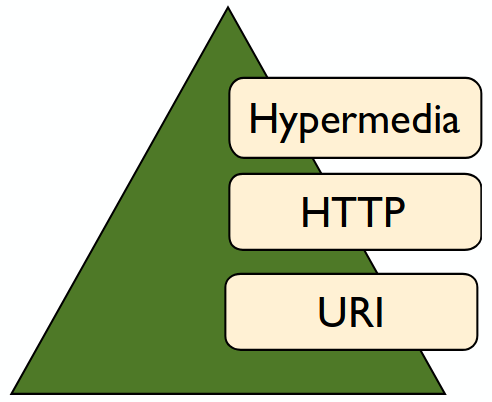
\includegraphics[width=0.25\columnwidth]{img/rmm}
\end{figure}
\begin{itemize}
\item Level 0: Don't use URIs or different methods. Usually use a single
URI.
\item Level 1: Use URIs to represent resources, but don't HTTP use methods.
\item Level 2: Use URIs and different methods, and return appropriate status
codes.
\item Level 3: Fully RESTful. Representations contain hyperlinks to other
resources. E.g. do a search for records rather than looking up a given
record.
\end{itemize}
\end{itemize}

\section{Continuous Delivery}

\paragraph{Agile Methods}

E.g. Extreme Programming, Scrum, Kanban. Favour an iterative approach
with \emph{small development cycles}.

\paragraph{Continuous Integration}

Developers should merge in work often to avoid integration problems.
Run automated tests to keep \texttt{master} healthy.
\end{document}
